\documentclass[border=4pt]{standalone}
\usepackage{times}
\usepackage[T1]{fontenc}
\usepackage{times}
\usepackage{latexsym}
\usepackage[utf8]{inputenc}
\usepackage{microtype}
\usepackage{graphicx}
\usepackage{tikz}
\usetikzlibrary{arrows.meta}
\definecolor{figblue}{HTML}{2A78D6}
\definecolor{figorange}{HTML}{EB6834}
\definecolor{figgray}{HTML}{6E6D69}
\usepackage{amsmath}
\usepackage{amssymb}
\usepackage{booktabs}
\usepackage{xcolor}
\newcommand{\todo}[1]{\noindent\textcolor{red!70!black}{\textbf{TODO:} #1}\par}
\newcommand{\tbd}[1]{\textcolor{red!70!black}{[#1]}}
\newcommand{\owner}[1]{\textcolor{blue!60!black}{\textsf{[#1]}}}
\newcommand{\donor}{\mathrm{D}}
\newcommand{\rec}{\mathrm{R}}
\usepackage{xspace}
\newcommand{\upd}[1]{\textcolor{blue}{#1}}
\newenvironment{updblock}{\color{blue}}{}
\newcommand{\gemmapt}{gemma-3-12b-pt\xspace}
\newcommand{\gemmait}{gemma-3-12b-it\xspace}
\newcommand{\mamay}{MamayLM\xspace}
\newcommand{\lapapt}{lapa-12b-pt\xspace}
\newcommand{\lapa}{lapa-v0.1.2-instruct\xspace}
\newcommand{\guard}{Llama-Guard-4-12B\xspace}
\begin{document}
  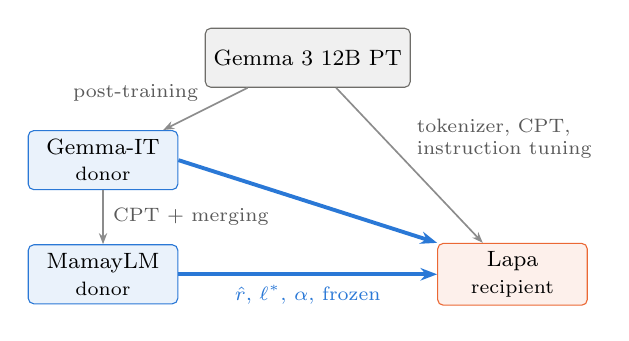
\begin{tikzpicture}[x=1cm,y=1cm,font=\footnotesize,
    model/.style={draw=#1, fill=#1!10, rounded corners=2pt, align=center, inner sep=3pt, minimum width=1.9cm, minimum height=0.75cm},
    train/.style={-{Stealth[length=4pt]}, draw=black!45, line width=0.6pt},
    borrow/.style={-{Stealth[length=6pt]}, draw=figblue, line width=1.4pt},
    lab/.style={font=\scriptsize, text=black!65}]
    \node[model=figgray] (pt) at (3.7,3.2) {Gemma~3 12B PT};
    \node[model=figblue] (it) at (1.1,1.9) {Gemma-IT\\{\scriptsize donor}};
    \node[model=figblue] (mam) at (1.1,0.45) {MamayLM\\{\scriptsize donor}};
    \node[model=figorange] (lapa) at (6.3,0.45) {Lapa\\{\scriptsize recipient}};
    \draw[train] (pt) -- node[lab, above left=-1pt] {post-training} (it);
    \draw[train] (it) -- node[lab, right] {CPT + merging} (mam);
    \draw[train] (pt) -- node[lab, above right=-1pt, align=left] {tokenizer, CPT,\\instruction tuning} (lapa);
    \draw[borrow] (it.east) -- (lapa.north west);
    \draw[borrow] (mam) -- node[lab, below, text=figblue] {$\hat r$, $\ell^{*}$, $\alpha$, frozen} (lapa);
  \end{tikzpicture}
\end{document}
